% Asset ID: A21TrigonometryAndModellingTikZ-005
% Purpose: Sinusoidal model annotated with amplitude, midline and period
\documentclass[tikz,border=10pt]{standalone}
\usepackage{amsmath}
\usetikzlibrary{arrows.meta,decorations.pathreplacing}
\begin{document}
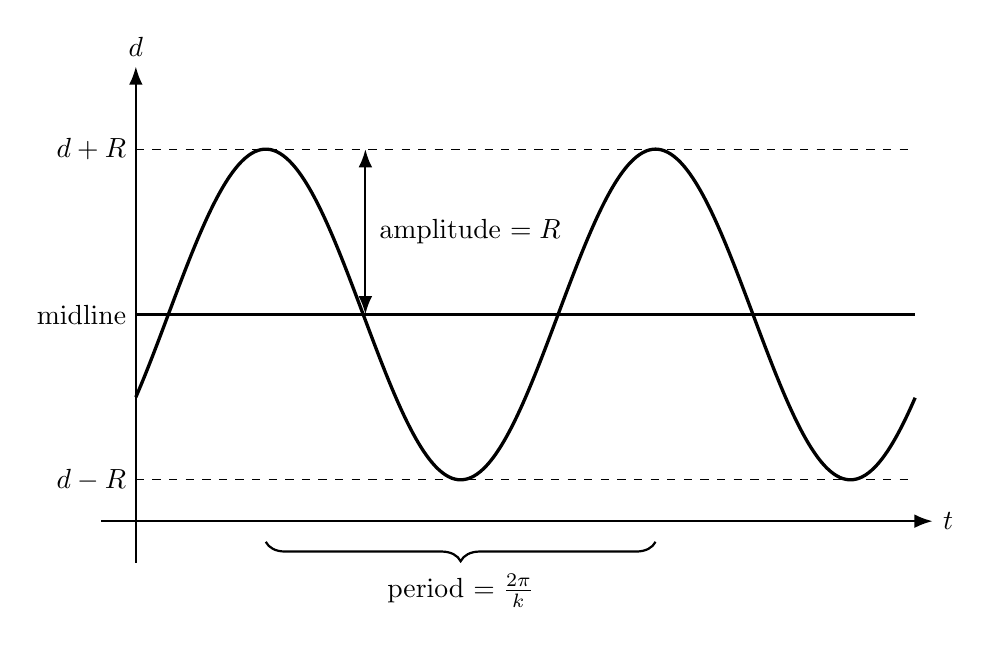
\begin{tikzpicture}[xscale=1.1,yscale=1.05]
\draw[-Latex,thick] (-0.4,0)--(9.2,0) node[right] {\(t\)};
\draw[-Latex,thick] (0,-0.5)--(0,5.5) node[above] {\(d\)};
\draw[thick] (0,2.5)--(9,2.5);
\draw[dashed] (0,4.5)--(9,4.5); \draw[dashed] (0,0.5)--(9,0.5);
\node[left] at (0,2.5) {midline}; \node[left] at (0,4.5) {\(d+R\)}; \node[left] at (0,0.5) {\(d-R\)};
\draw[very thick,domain=0:9,smooth,samples=250] plot (\x,{2.5+2*sin((\x*80)-30)});
\draw[Latex-Latex,thick] (2.65,2.5)--(2.65,4.5); \node[right] at (2.7,3.5) {amplitude \(=R\)};
\draw[decorate,decoration={brace,mirror,amplitude=7pt},thick] (1.5,-0.25)--(6.0,-0.25) node[midway,below=8pt] {period \(=\frac{2\pi}{k}\)};
\end{tikzpicture}
\end{document}
